% Created 2016-02-07 Sun 17:55
\documentclass[11pt]{article}
\usepackage[utf8]{inputenc}
\usepackage[T1]{fontenc}
\usepackage{fixltx2e}
\usepackage{graphicx}
\usepackage{longtable}
\usepackage{float}
\usepackage{wrapfig}
\usepackage{rotating}
\usepackage[normalem]{ulem}
\usepackage{amsmath}
\usepackage{textcomp}
\usepackage{marvosym}
\usepackage{wasysym}
\usepackage{amssymb}
\usepackage{hyperref}
\tolerance=1000
\usepackage{setspace}
\singlespacing
\usepackage[margin=1in]{geometry}
\usepackage{enumitem}
\setlist[enumerate,itemize]{noitemsep,nolistsep,leftmargin=*}
\usepackage[notes,isbn=false,backend=biber]{biblatex-chicago}
\addbibresource{main.bib}
\author{Jason Dempsey}
\date{}
\title{RISCV CPU in Synthesizable VHDL}
\hypersetup{
  pdfkeywords={},
  pdfsubject={},
  pdfcreator={Emacs 25.0.50.1 (Org mode 8.2.10)}}
\begin{document}

\maketitle


\section{Introduction}
\label{sec-1}
This project is a 4-stage pipeline, Reduced Instruction Set Computer-5 (RISCV) Instruction Set Architecture (ISA) utilizing branch prediction and a dedicated caching scheme. The 4 stages within the pipeline are Instruction Fetch (IF), Instruction Decode (ID), Execute (Ex), and Writeback or Store (ST).

\section{Part Choice}
\label{sec-2}
For this project, I will be using the DE0 nano Development and Education Board as the main development platform. It supports 56 M9k (8192 byte) internal memory blocks as well as an SDRAM module of 32 MB in size. With approximately 22,000 logic elements, the entire CPU design will fit.
\section{Implementation}
\label{sec-3}
Adhering to the RISC-V V2.0 specification, the standard word size will be 32-bits and will consist of 32 general purpose registers, each of which is 1 word in size. An additional register will be used to store the value of the program counter, which is only accessible through one instruction in the general ISA\footnote{: \url{http://riscv.org/download.html#tab_spec_user_isa}}.


\subsection{Pipeline}
\label{sec-3-1}

\begin{figure}[htb]
\centering
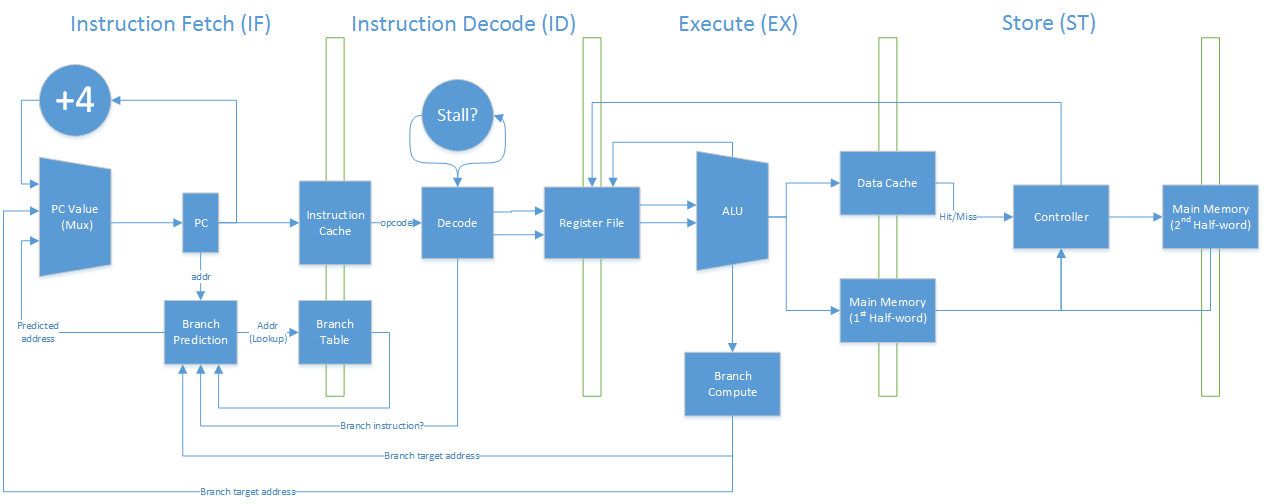
\includegraphics[width=.9\linewidth]{./bd.png}
\caption{\label{fig:pipeline}Pipeline Diagram}
\end{figure}

\subsubsection{Instruction Fetch}
\label{sec-3-1-1}
In this stage, the program counter is updated based on either a predicted branch, a true branch, or simply incremented. From here, the next instruction is looked up in the Data Cache, based on the counter value. Simultaneously, the branch prediction module will receive the Program Counter's value and decide whether or not, based off of branch history, whether or not that address is a branch or not, and will attempt to predict the next address that should be processed. Refer to Section \ref{SEC:BranchPrediction} for more information.
\subsubsection{Instruction Decode}
\label{sec-3-1-2}
Here, the instruction is decoded. If registers are required to perform the operation in the next stage, those register addresses are output to the register file to be read from on the next clock boundary.
\begin{enumerate}
\item Hazard Detection / Mitigation:
\label{sec-3-1-2-1}
If a load or store instruction is decoded, a 1-cycle penalty will be incurred within the pipeline. To account for this, a 'bubble' (NOP instruction) is inserted into the pipeline. The Program Counter will not increment for one cycle and the NOP will pass through the pipeline.
\end{enumerate}
\subsubsection{Execute}
\label{sec-3-1-3}
In the execute phase, the instruction is actually executed here. The ALU processes the values from the register file. It may be necessary to fully compute a branch instruction here. Once done, this target address is returned to both the Program Counter as well as the Branch Predictor, so that both values may be updated. 
If a load was decoded in the previous cycle, cache and main memory will be read from on the next clock boundary, as described in Section \ref{SEC:Store}.
A Store will incur a similar process.

\subsubsection{Store / Writeback}
\label{sec-3-1-4}
\label{SEC:Store}
    If a value is required to be retrieved from memory (a load operation), it will be performed in this stage. When the memory  controller detects a cache miss, it must request the necessary data from main memory (SDRAM). A further issue is created due to the SDRAM supporting only half-word read/writes. To mitigate pipeline stalling as much as possible, while the data cache is read, so will the first half-word from main memory. Therefore, if a cache miss does occur, it will not incur a 2-cycle penalty, but only 1 further cycle, for the additional half-word. Once either the cache has found the data, or has been retrieved from main memory, it can be written to the resulting register.

If a load is requested, a similar process occurs.  

\subsection{Main memory}
\label{sec-3-2}
Main memory will reside on the SDRAM module. A memory controller module will be required to either write to, or read from, the SDRAM itself. This will be generated by either a megafunction within Quartus, or from an external entity and given the proper credit.

\subsection{Data Cache}
\label{sec-3-3}
The caching scheme that will be used will be a 2-way set associative cache\footnote{: \url{http://csillustrated.berkeley.edu/PDFs/handouts/cache-3-associativity-handout.pdf}}. This method extracts the last bits from the LSB as a tag to perform a lookup for the specific data, associated with that tag. If it is found, it is a cache hit and can be returned, if not, it is a cache miss and the pipeline must wait on the SDRAM, in this case main memory, to retrive the piece of data.

\subsection{Branch Prediction}
\label{sec-3-4}
\label{SEC:BranchPrediction}
Branch Prediction is generallly used within a RISC pipeline to mitigate a pipeline flush which can be a source of delay within execution of a program. Modern pipelines may consist of 10 to 20 stages, so a flush could be extremely expensive, resulting in 10's of clock cycles in delay.

\subsubsection{Implementation}
\label{sec-3-4-1}
The prediction scheme will be a 'bimodal' prediction algorithm\footnote{: \url{https://www.cs.york.ac.uk/ftpdir/papers/rtspapers/R:Bate:2005b.pdf}}. While one of the simplest, it's success rate is high in comparison with much more advanced prediction schemes\footnote{: \url{http://web.engr.oregonstate.edu/~benl/Projects/branch_pred/#l6}}. A lookup will consist of the current Program Counter value acting as the 'tag' to lookup the resulting data. If the tag is found, this data will consist of a two bit value which yields a 4-state state machine as described in the following table:

\begin{center}
\begin{tabular}{rl}
Value & Usage\\
\hline
00 & 'Strongly' Not Taken\\
01 & 'Weakly' Not Taken\\
10 & 'Weakly' Taken\\
11 & 'Strongly' Taken\\
\end{tabular}
\end{center}

As well as the target address to branch to. 

If the data is not found, the branch predictor will not output a value for the given instruction.

Once the instruction has been decoded, the decoder will inform the predictor if that address is one which is a branch. If so, and once the branch target address is fully computed within the Execute stage, the predictor will update its lookup table accordingly with the given values.

\section{C to Assembly Interface}
\label{sec-4}
A goal of this project is to be able to develop a program in C, and have it be compiled down to the RISC-V Assembly set. Once this happens, this program may be loaded into the cache as the new program to be ran by the FPGA.

\subsection{Details}
\label{sec-4-1}
To accomplish this task, this project will use the C/C++ compiler Clang which is built on the Low Level Virtual Machine (LLVM). Clang is different from other C/C++ compilers (VC++, GCC, etc.), in that it does not compile higher level code down to the machine level (or binaries). Instead, Clang compiles down to an intermediate bytecode which the LLVM can interpret and write assembly or binaries based off of this bytecode for a specific architecture. This allows developers to target multiple architectures (x86, Itanium, ARM, etc.) with a singular codebase.

A RISC-V instruction set extension is supported in the LLVM, allowing this project to take C and convert it into RISC-V assembly. Loading a new program onto the FPGA will require resynthesis of the project, this is a limitation of the FPGA itself.

\section{Development}
\label{sec-5}
\subsection{Initial}
\label{sec-5-1}
Development will initially take place in a simulation tool (ModelSim). Once a basic pipeline has been created and verified, the synthesizable codebase will be moved to Quartus to be developed further on the FPGA hardware.

Branch prediction, cache, and pipeline development will happen somewhat independently. If their interfaces are defined early and adhered to through the development process, they can be developed at different points within the lifecycle.

\subsection{Timing Constraints}
\label{sec-5-2}
Timing analysis will be taken into account once a basic pipeline has been implemented. Analysis of the critical path through the pipeline will take place through Quartus' TimeQuest tool. The goal is for no slower than 50 MHz.
% Emacs 25.0.50.1 (Org mode 8.2.10)
\end{document}